\question \textbf{Ford-Fulkerson}

\begin{parts}
\part  Use the Ford-Fulkerson algorithm to find a maximum flow in the network.

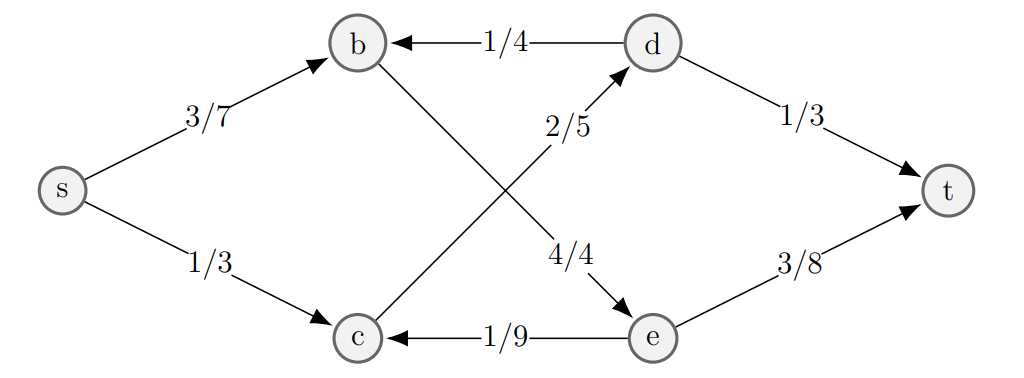
\includegraphics[width=0.6\linewidth]{task_2/task_2.pdf}

\begin{solution}
Here goes the solution
\end{solution}


\part Find a minimum cut proving the maximality of the flow.


\begin{solution}
Here goes the solution
\end{solution}

\end{parts}


% For tasks without simply remove the \begin{parts}...\part...\end{parts} commands